\chapter{Požadavky}
voděodolnost


\chapter{Základní návrh}
%tady musí být text
%bude tady také blokové schéma

\section{Bezdrátová komunikace}
Použití na táborech a outdoorových akcích vyřadilo z výběru drátovou komunikaci. K DPS by muselo být ještě velké množství kabelů 
o délce několika stovek metrů minimálně. Bezdrátová komunikace je z tohoto hlediska velmi praktická. Je to také moderní řešení 
náležící dnešní době. 

Jedním ze základních požadavků bylo, že jednotlivé DPS mezi sebou musí být schopny komunikovat. Vzhledem k použití na táborech 
musel být vybrán komunikační protokol a následně k němu přizpůsoben hardware. 

Práce tedy započala tím, že byla udělána rešerše existujících bezdrátových komunikačních protokolů a následně byly tyto protokoly 
mezi sebou porovnány. Vzhledem k použití na outdoorových akcí byl kladem důraz na komunikační vzdálenost a náročnost na výkon, 
jelikož zařízení je napájeno z baterií. 

\subsection{WiFi}
Komunikace pomocí WiFi sítě je jednou z nejznámějších a nejpoužívanějších bezdrátových komunikací užívaných širokou veřejností. 
WiFi je dnes na každém pracovišti, na veřejných místech i v každé domácnosti. Využívána je především k připojení k internetu. 
Přes WiFi lze přenášet velké objemy dat vysokou rychlostí. Pracuje v pásmech v okolí frekvencí 2,4 GHz a 5,0 GHz s dosahem 
desítek až nižších stovek metrů \cite{Bezdrat_muni}.
%doplnit

Výhody bezdrátové technologie WiFi jsou \cite{Bezdrat_muni}:
\begin{itemize}
  \item pracuje v bezlicenčním pásmu, %doplnit do textu
  \item levná, %doplnit do textu
  \item velmi rozšířená.
\end{itemize}

Nevýhody jsou \cite{Bezdrat_muni}:
\begin{itemize}
  \item omezený výkon (není možné pokrýt rozáhlejší oblasti), %doplnit do textu
  \item vyšší spotřeba energie.
\end{itemize}
%doplnit

\subsection{Bluetooth}
Bluetooth je také velmi rozšířenou technologií bezdrátové komunikace. V dnešní době rozšířené WiFi komunikace je ale na ústupu. Používá 
se na přenos dat na krátké vzdálenosti. Běžně se využívala pro přenos fotografií z jednoho zařízení do druhého apod. V dnešní době se
spíše využívá pro připojení bezdrátových periferií jako jsou bezdrátová sluchátka, myši a klávesnice. Tato technologie je zaměřena 
především na nízkou spotřebu, i proto je komunikační vzdálenost maximálně 100 metrů \cite{Bezdrat_muni}. V praxi jde ale o nižsí desítky
metrů. Bluetooth je také technologií pro propojení pouze 2 zařízení, kde jedno je tzv. master a druhý tzv. slave \cite{Bezdrat_muni}. 
Jedno zařízení je tedy nadřazeno druhému. V případě telefonu a sluchátek je telefon nadřazený sluchátkům. 
%doplnit

Výhody bezdrátové technologie Bluetooth jsou \cite{Bezdrat_muni}:
\begin{itemize}
  \item nízká spotřeba.
\end{itemize}

Nevýhody jsou \cite{Bezdrat_muni}:
\begin{itemize}
  \item krátký dosah,
  \item možnost propojení pouze 2 zařízení.
\end{itemize}
%doplnit

\subsection{NFC}
NFC je jedna z novějších technologií, která se používá převážně při platbě kartou. Jde tedy o přenos malých objemů dat na velmi krátkou 
vzdálenost, tj. do desítek centimetrů \cite{Bezdrat_muni}. NFC je technologií, kde stačí, aby pouze jedno zařízení mělo zdroj elektrické 
energie \cite{Bezdrat_muni}. Druhé zařízení se chová jako anténa, ze které je možné vyčíst informace \cite{Bezdrat_muni}. Například při 
platbě kartou v sobě karta nemá žádný zdroj energie, ale při přiložení k terminálu je pomocí elektromagnetické indukce vyčteno identifikační
číslo karty. Díky tomu je možné zaplatit. 
%doplnit

Výhody bezdrátové technologie NFC jsou \cite{Bezdrat_muni}:
\begin{itemize}
  \item rychlost, %doplnit do textu
  \item možnost interakce se zařízeními bez vlastního zdroje elektrické energie.
\end{itemize}

Nevýhody jsou \cite{Bezdrat_muni}:
\begin{itemize}
  \item velmi krátká komunikační vzdálenost,
  \item možnost komunikace pouze mezi dvěma zařízeními, 
  \item nízká rychlost přenosu,
  \item malý objem přenášených dat.
\end{itemize}
%doplnit
%doplnit do zkratek NFC (Near Field Communication), WiFi (Wireless Fidelity)

\subsection{ZigBee} %mozna cele smazat
ZigBee technologie je používána pro vytvoření malých sítí, kde může signál snadno přeskakovat z jednoho zařízení na druhé \cite{ZigBee_smart}.
Není přitom zapotřebí, aby bylo každé zařízení připojeno k internetu pomocí WiFi \cite{ZigBee_smart}. Pro komunikaci je ale zapotřebí centrální 
rozbočovač, kterž zajišťuje komunikaci mezi zařízeními \cite{ZigBee_smart}. Tato technologie je určena pro tvorbu rozsáhlejších bezdrátových sítí
s přenosem menšího objemu dat \cite{ZigBee_smart}. Jedná se o spolehlivou technologii s nenáročnou implementací a nízkou spotřebou elektrické energie 
\cite{ZigBee_smart}. Díky ZigBee může mít uživatel v jedné aplikaci zařízení 
od různých značek a výrobců, protože právě ZigBee zajišťuje jejich vzájemnou komunikaci \cite{ZigBee_smart}.
%doplnit

Výhody bezdrátové technologie ZigBee jsou \cite{ZigBee_smart}:
\begin{itemize}
  \item nízká spotřeba elektrické energie,
  \item spolehlivost, 
  \item nenáročná implementace.
\end{itemize}

Nevýhody jsou \cite{ZigBee_smart}:
\begin{itemize}
  \item nutnost centrálního rozbočovače.
\end{itemize}
%doplnit

%Velká přehledová tabulka s důležitými údaji od každého protokolu, aby bylo jasné, proč byla vybrána LoRa.

\section{Mikrokontrolér}
Faktory ovlivňující výběr řídicího mikrokonroléru:
\begin{itemize}
  \item dostatečný počet GPIO pinů,
  \item dostatek paměti,
  \item WiFi,
  \item ADC,
  \item cena,
  \item periferie pro připojení Lora modulu.
\end{itemize}

%do zkratek ZigBee, GPIO, ADC
Dostatečný počet GPIO %specifikovat minimum
Dostatek paměti %lépe specifikovat
WiFi
ADC %pro senzor pro osvětlení
Cena %rozumné hranice
Periferie pro připojení pro LoRa modul

Nice to have:
USB rozhraní (nemusel by být použit převodník)
Možnost režimu spánku %možná nepsat


Jedním z požadavků na mikrokonrolér byla zabudování WiFi. Asi nejznámnějšími mikrokonroléry s WiFi jsou ESP32 od firmy 
Espressif. Mikrokontroléry ESP32 jsou dostupné v různých variantách, ale všechny mají WiFi a dělají se i ve variantách 
se zabudovanou anténou. 
%proč jsem vybrala ESP
%proč právě tento typ 
%napsat přesné označení čipu - dále ž jen ESP32-C3

Rozsah napájecího napětí je 3 až 3,6 V \cite{ESP_C3_dtsh}.
%jaké má periferie

\section{LED}
Jendím z nejdůležitějších požadavků na Semafor je, aby mohl svítit. Čím více možností, jak svítit, tím bude využití 
při hrách a táborových programech větší. K tomu jsou použity LED. Obyčejné LED mají pouze jednu barvu, kterou 
mohou svítit. Existují také RBG LED, ale ty mají 4 vývody a každá LED tak zabírá 3 GPIO piny mikrokontroléru - jeden pin
pro jednu barvu. K tomu by byl zapotřebí mikrokonrolér s velkým množství GPIO pinů a jeho programování by se tím značně 
komplikovalo. Ani to není žádoucí, a proto byly použity programovatelné LED typu WS2812C.

Tyto programovatelné LED WS2812C lze spojovat za sebe, takže datový výstup jedné LED je připojen k datovému vstupu další 
LED \cite{WS2812C_dtsh}. Takto lze spojit nekonečné množství těchto programovatelných LED a připojit je na jeden GPIO pin MCU. 
Každá LED má pin pro vstupní napětí, GND, vstupní datový pin a výstupní datový pin. 

Napájecí napětí těchto LED by se mělo pohybovat v rozmezí 4,5 až 5,5 V \cite{WS2812C_dtsh}. Kondenzátor u každé LED slouží pro 
filtraci napájecího napětí. 

%způsob programování (jak funguje použitá knihovna?)

%obrázek spojení LED za sebe

Komunikační napěťová úroveň logické jedničky těchto LED by měla být alespoň na úrovni 70 \% napájecího napětí \cite{WS2812C_dtsh}. 
Protože použitý mikrokonrolér ESP32-C3 má komunikační napěťovou úroveň logické jedničky jeho napájecí napětí, což je 3 až 3,6 V, 
tak je zapotřebí využít převodník napěťové úrovně \cite{ESP_C3_dtsh}. Komunikace je v tomto případě pouze jednosměrná, 
to znamená, že MCU posílá data do LED, ale LED neposílají žádná data do MCU. Převodník je realizován unipolárním tranzistorem 
a jedním pullup rezistorem. Rezistor je připojen pro k napájecímu napětí inteligentních LED WS2812C. 
Tranzistor Q1 má gate připojený k napájecímu napětí MCU. Pokud bude mikrokonrolér do LED posílat logickou jedničku, tak bude rozdíl
mezi gate a source 0 V. Tím pádem bude tranzistor uzavřený a tím se přes rezistor R4 připojí k LED jejich napájecí napětí. Toto napětí 
je pro inteligentní LED logickou jedničkou. Pokud bude MCU posílat logickou nulu, tedy 0 V, tak je rozdíl napětí mezi gate a source 
napájecí napětí mikrokontroléru. Tranzistor je tedy otevřený a tím se napětí 0 V dostane k inteligentním LED a na rezistoru se objeví
úbytek napětí o velikosti napájecího napětí inteligentních LED. Napětí 0 V je logickou nulou i pro inteligentní LED. Tento převodník
je určen pouze pro komunikaci jedním směrem. 

%schéma převodníku 

Tyto programovatelné LED mají maximální spotřebu 5 mA na jeden kanál. Při zapnutí všech kanálů (svícení bílou) je maximální
spotřeba jedné LED 15 mA \cite{WS2812C_dtsh}. Pokud LED nesvítí, tak je její maximální klidový proud 0,3 mA \cite{WS2812C_dtsh}.
Při použití 12 LED je tedy maximální odběr všech LED 180 mA.

%do sekce o DPS se zmínit o jejich umístění - kruh, hodiny, proto 12 ks. (lze také rozdělit na 3 segmenty)



\section{Tlačítka}
Tlačítka jsou nezbytnými prvky pro ovládání Semaforu. Mohou sloužit pro přepínání módů, ovládání Semaforu jako takového nebo jako herní 
součást. Ve hře mohou plnit úlohu přepínače režimů hry, zadávání kódů, určování směru apod. 

Tlačítka mohou být realizována dvěma základními způsoby, mohou být elektromechanická, nebo kapacitní dotyková. 

Dotyková plocha mechanického tlačítka je nevodivá, často plastová. 

Mechanické tlačítko typu NO: %upravit

Po zmáčknutí mechanického tlačítka jsou 2 kovové části tlačítka spojeny, tím dochází ke spojení elektrického obvodu 
a odpor smyčky je v ideálním případě nulový. Tlačítko je tedy sepnuto. Když je tlačítko rozpojeno, tak je 
elektrický obvod přerušen a odpor smyčky je v ideálním případě nekonečný.

Mechanické tlačítko typu NC: %upravit

U tlačítka NC je to přesně naopak. %upravit

%sem přidat fotku vnitřku mechanického tlačítka

Kapacitní tlačítka jsou tvořena měděnou vrstvou a nejsou nijak mechanicky namáhána. Tlačítko může být zmáčknuto i přes 
obal krabičky, a proto může být celé zařízení mechanicky odolné i voděodolné. 

Nevýhodou kapacitních tlačítek je, že nemají žádnou odezvu na dotyk. U mechanických tlačítek je odezvou samotný fyzický 
stisk tlačítka. U kapacitních tlačítek lze tento fakt vyřešit například rozsvícením LED nebo vibrační odezvou. Vibrační 
odezva může být realizována pomocí vibračního motoru. Některé MCU včetně vybraného mikrokontroléru ESP32-C3 nemají kapacitní
vstupy, to znamená, že tlačítko nelze připojit přímo k pinu MCU. Buď musí být vybrán mikrokonrolér, který kapacitní vstupy má,
nebo může být použit převodník, který má kapacitní vstupy a jeho výstupy poté mohou být připojeny k MCU. 

V návrhu Semaforu byla zvolena kapacitní dotyková tlačítka. Pro možnost použití uvnitř i venku jsou díky možnosti voděodolnosti 
vhodnějším řešením. Také označení tlačítka může být variabilní, protože může být na DPS v místě tlačítka vyznačeno barevně, nebo 
např. samolepkou. Odezva na dotyk se realizuje pomocí vibračního motoru. Ke čtení dotykových tlačítek je využit převodník. 

\subsection{Princip kapacitních dotykových tlačítek}
Základní princip je založen na měření změny kapacity. Měď, ze které je tlačítko vytvořeno má
nějakou vlastní kapacitu (kapacita samotné nosné desky) a po přiložení prstu je kapacita zvýšena o paralelně 
připojenou kapacitu přechodu tlačítka a prstu díky obsahu železa v krvi a vodivosti kůže \cite{PrincipKapTl}. 
Prst se tedy chová jako druhá uzemněná elektroda \cite{PrincipKapTl}. 

Kapacita snímače se tedy volí co nejmenší, aby přiložený prst vyvolal co nejvetší změnu kapacity. Ve snímači se vyskytuje
RC článek, kterého se mění doba nabíjení kondenzátoru a tím je možné detekovat stisk tlačítka \cite{PrincipKapTl}. 

\subsection{Návrh kapacitního dotykového tlačítka}
Tvar tlačítka nemá vliv na schopnost detekce dotyku \cite{PrincipKapTl}. Naopak velký vliv má plocha tlačítka, tloušťka
izolační vrstvy, a také vzdálenost jednotlivých tlačítek od sebe \cite{PrincipKapTl}. 

Čím větší je plocha tlačítka, tím je větší změna kapacity při dotyku a díky tomu je vytvořena lepší schopnost detekce 
dotyku \cite{PrincipKapTl}. S rostoucí tloušťkou izolační vrstvy se naopak schopnost detekce dotyku snižuje \cite{PrincipKapTl}.

Pokud jsou tlačítka příliš blízko u sebe, tak může docházet k jejich vzájemnému ovlivňování. Kvůli tomu pak může docházet k
detekci dotyku špatného tlačítka, nebo k falešné detekci dotyku. Z doporučení plyne, že pro dotyk prstu je vhodná velikost snímací 
plochu pro prst 13~$\times$~13 mm a jejich vzdálenost alespoň 5 mm od sebe \cite{PrincipKapTl}. Proti vzájemnému ovlivňování tlačítek
se používají uzemňovací meziplošky \cite{PrincipKapTl}. 

%sem dát obrázek, kde je ukázán návrh GND meziplošek

U kapacitních dotykových tlačítek je zapotřebí dbát na správné připojení k MCU. U vícevrstvých DPS nesmí pod tlačítky, ani pod přívody
k MCU, vést jiné dráhy, ani se zde nesmí vyskytovat jiné součástky \cite{PrincipKapTl}. Součástky nesmí být ani z vrchní, ani ze spodní 
strany DPS \cite{PrincipKapTl}. Přívody kapacitních tlačítek k MCU by měly být odstíněny pomocí GND signálu.

Voda a další nečistoty mění vlastní kapacitu tlačítka a může tak docházet k falešným stiskům tlačítka. Tento problém lze řešit softwarově. 
Lze využít faktu, že nečistoty působí dlouhodobě, ale stisk je krátkodobý \cite{PrincipKapTl}. Hodnotu vlastní kapacity tlačítka je tedy
možné softwarově upravovat v závislosti na aktuálních dlouhodobějších stavech a detekovat tak přesněji krátkodobý stisk tlačítka.

%dát do zkratek MCU, DPS, GPIO, LED, GND

%\begin{figure}[!h]
%    \begin{center}
%      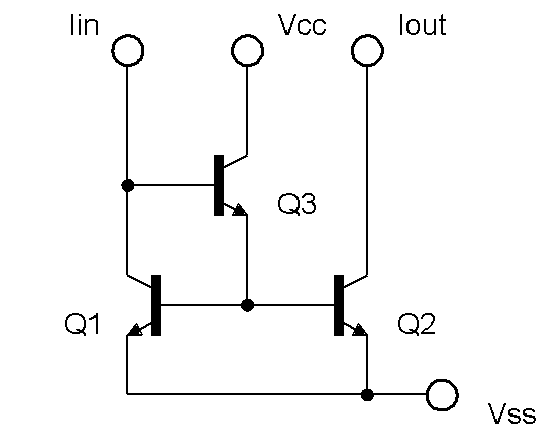
\includegraphics[scale=0.5]{obrazky/ZlepseneWilsonovoZrcadloNPN}
%    \end{center}
%    \caption[Alenčino zrcadlo]{Zlepšené Wilsonovo proudové zrcadlo.}
%  \end{figure}

Pro odlišení tlačítek je místo označeno barevným potiskem. 

\section{Vibrační motor}
Vibrační motory jsou založeny na principu kmitání. Motor je připevněn k zařízení, které je kmitáním rozvibrováno. Vibrační motory jsou dnes 
nedílnou součástí mnoha elektronických zařízení včetně mobilního telefonu nebo dětských hraček. 

Dioda slouží jako ochrana proti přepětí, protože motor je indukční zátěž, takže vytváří napěťové špičky. Díky diodě je mikrokonrolér chráněn 
proti špičkovému napětí, které by se na něj mohlo dostat. Kondenzátor slouží k tomu, aby napěťové špičky eliminovat, nebo alespoň zmenšoval. 

Vibrační motor je připojen k mikrokontroléru přes tranzistor, protože maximální výstupní proud z pinu MCU není dostatečně velký na to, aby 
motor roztočil. Tranzistor je tedy připojen na gate tranzistoru, který se při logické jedničce na pinu sepne a motorem protéká proud, který 
nedodává MCU, ale zdroj 3.3 V (v tomto případě baterie LiFePO4). Baterie tak dokáže dodat dostatek proudu, aby se motor roztočil. 

Pro Semafor byl vybrán vibrační motor LCM1020A2945F. Tento motor má maximální požadovaný proud 120 mA \cite{vib_motor_dtsh}. Maximální proud, 
který lze odebírat z pinu mikrokontroléru ESP32-C3, je 40 mA \cite{ESP_C3_dtsh}. Vibrační motor lze pouze spínat, nebo je možné jej připojit 
k pinu, který dokáže generovat PWM a lze tím regulovat jeho otáčky. 

Vibrační motor slouží jako odezva na dotyk kapacitního tlačítka. 

%obrázek schéma zapojení + asi fotka vybraného motoru

\section{Převodník pro kapacitní tlačítka}
Vybraný mikrokonrolér ESP32-C3 nemá kapacitní vstupy, proto je zapotřebí kapacitní dotyková tlačítka připojit přes převodník. Je zapotřebí připojit 
5 tlačítek. 
%jaké byly možnosti 
%zmínit se i o TTP224?
%má 4 vstupy, ale já potřebuji 5 tlačítek

Použitý převodník AT42QT1070 dokáže pracovat ve 2 režimech. V prvním režimu může být zapojeno maximálně 5 kapacitních tlačítek, která jsou připojena
k pinům KEY0 až KEY4. Jako výstup se používají piny OUT0 až OUT4. Každé tlačítko má tedy svůj výstup, který může být připojen k GPIO pinům MCU 
nebo k nim mohou být připojeny např. LED \cite{conv_cap_but_AT42QT1070_dtsh}. 

Druhý režim je využitelný pouze v případě, je-li převodník připojen k MCU. Vtomto případě může být k převodníku připojeno až 7 kapacitních tlačítek, 
která jsou připojena na pinech KEY0 až KEY6. Převodník poté komunikuje s MCU pomocí komunikační sběrnice I2C \cite{conv_cap_but_AT42QT1070_dtsh}. 
Z registru převodníku lze poté vyčíst stavy daných kapacitních dotykových tlačítek. 

Jelikož je v tomto návrhu Semaforu využit mikrokontrolér, který podporuje komunikaci po sběrnici I2C, tak bylo využito právě zapojení s komunikací 
přes I2C. Díky tomu budou využity pouze 2 GPIO piny mikrokonroléru ESP32-C3 a ne 5 GPIO pinů, které by byly zapotřebí při zapojení bez komunikace pro
sběrnici I2C.

Převodník má kondenzátory C3 a C4 připojeny na napájecím pinu vůči zemi, aby nebyly případné proudové špičky přivedeny na napájení převodníku. Rezistory
R17 a R18 slouží jako pullup rezistory při komunikaci pomocí sběrnice I2C s mikrokonrolérem EP32-C3. Na piny KEY0 až KEY4 jsou připojena kapacitní 
dotyková tlačítka.  
%proč je MODE na zemi
%proč nepoužívám pin /CHANGE?
%obrázek - schéma


\section{Baterie}
Ve výběru baterií hraje velkou roli kapacita, napětí, velikost a cena. Požadavkem je také možnost nabíjení, protože není žádoucí, aby si uživatel
baterie měnil. Při použití na táboře by také musely být stále nové baterie v balení a musely by se neustále doplňovat a udržovat.)
%další důvody, proč nabíjecí baterku

%kapacita baterie - jak dlouho by měla vydržet

Vybraný mikrokonrolér má napájecí napětí v rozsahu 3 až 3,6 V \cite{ESP_C3_dtsh}. 

Z nabíjecích baterií je možno vybírat z nabíjecích tužkových baterií (Ni-MH), Li-Ion, Li-Pol a LiFePO4 baterií.
%Ni-MH
Baterie Ni-MH mají jmenovité napětí 1,25 V. %citace
Proto by bylo zapotřebí alespoň 3 článků spojených sériově, u kterých by navíc musel být stabilizátor
na 3,3 V pro napájení mikrokontroléru. % a co inteligentní LED?
%Li-Ion

%Li-Pol

%LiFePO4
LiFePO4 baterie mají jmenovité napětí v rozsahu %xyz V + citace.



\section{Nabíjecí obvod}
Nabíjecí obvody jsou závislé na konkrétním typu baterií, které budou nabíjeny. Vzhledem k vybranému typu baterií LiFePO4 byly uvažovány pouze komerčně
dostupné integrované obvody, které jsou určeny pro nabíjení tohoto typu baterií. 
%ještě TP5000 zmínit? - zkontrolovat jestli je opravdu na pro LiFePO4

Vybraný typ baterií LiFePO4 lze nabíjet pomocí obvodu CN3058E \cite{charger_dtsh}. 
%možná vyjmenovat další obvody a napsat proč tento

%napětí nastaveno na 3,6 V interně, ale lze jej nastavit pomocí externího odporu
%nabíjecí proud se nastavuje externím rezistorem - není využito
%při odpojení napájecího napětí přechází tento obvod do režimu spánku, takže je baterie vybíjena proudem menším než 3 uA
%lze snímat teplotu na baterii

Nabíjecí obvod CN3058E je určen pro nabíjení pouze LiFePO4 baterií a lze jím napájet právě 1 článek těchto baterií \cite{charger_dtsh}. Napájecí napětí tohoto 
nabíjecího čipu se pohybuje mezi 3,8 až 6 V \cite{charger_dtsh}. Díky tomu lze přímo použít napětí z USB konektoru. 

%popsat další vlastnosti 

%doporučené schéma zapojení čipu - z datasheetu

Tento nabíjecí obvod se vyrábí ve standardizovaném pouzdře SOP8 \cite{charger_dtsh}.

\subsection{Zapojení nabíjecího obvodu}
Rezistor připojený k pinu ISET slouží pro nastavení hodnoty nabíjecího proudu \cite{charger_dtsh}. V tomto zapojení byl počítán pro nabíjecí proud 1 A. 

%1218/1 = 1218 Ohm
%rovnici + citace

Z výpočtu vyplývá, že rezistor by měl mít hodnotu 1218 $\Omega$. Nejbližší hodnota z rezistorové řady E12 je hodnota 1,2 k$\Omega$, proto byl také zvolen rezistor 
o této hodnotě \cite{rezistorova_rada}. Odpovídá tomu nabíjecí proud 1015 mA, který nebude mít vliv na životnost baterií. 

%rovnice 1218/1200 = 1.015 A = 1015 mA

Vstupní a výstupní kondenzátory slouží pro filtaci zákmitů napájecího napětí a také napětí, kterým je nabíjena baterie. Hodnoty kondenzátorů byly převzaty
z doporučení z datasheetu.

Kladný pól nabíjené baterie je připojen na pinu BAT, záporný pól je připojen ke GND. 
%do zkratek přidat GND

Tento nabíjecí obvod má možnost indikace nabíjení baterií a dokončení nabíjení. Tato indikace je realizována pomocí 2 LED připojených přes pullup rezistor. Hodnota
pullup rezistoru byla převzata z doporučení z datasheetu. Červená LED indikuje nabíjení baterií a je připojena na pin /CHRG a zelená LED indikuje dokončené nabíjení 
a je připojena na pin /DONE. Obě LED jsou k pinům nabíjecího čipu připojeny katodou. 

Obvod CN3058E může také měřit teplotu na nabíjené baterii. Slouží k tomu pin TEMP. Měření probíhá pomocí odporového děliče, jehož střed je připojen na snímač teploty. 
Tento snímač je připojen na baterii. V této práci není měření teploty baterií využíváno, a proto není pin obvodu TEMP nikam připojen. 

%obrázek z datasheetu, kde je připojeno i meření teploty

Pokud není baterie nabíjena, tak by svodový proud pinu BAT nabíjecího obvodu CN3058E vibíjel baterii. Svodový proud tohoto pinu je 3 $\mu$A \cite{charger_dtsh}. 
Aby se baterie zbytečné navybíjela, tak je do obvodu připojen tranzistor Q2, který detekuje připojené napětí k nabíjecímu obvodu. Pokud je napětí připojeno, tak je 
tranzistor otevřen a baterie je nabíjena. Pokud napětí připojeno není, tak je tranzistor uzavřen a baterie je díky tomu odpojena od nabíjecího obodu. Díky tomu 
není vybíjena svodovým proudem pinu BAT. 

\section{Zvyšovač napětí pro LED}
Pro napájení vybraných inteligentních LED je zapotřebí napětí v rozsahu 4,5 až 5,5 V \cite{WS2812C_dtsh}. Použité baterie LiFePO4 mají napětí pouze 3,2 V, proto je 
zapotřebí použít zvyšovač napětí. 

Z komerčně dostupných integrovaných obvodů byl hledán zvyšovač napětí, který vytváří z napětí 3,3 V napětí 5 V a dodávat přitom do výstupu proud alespoň 200 mA. 
Maximální odběr všech 12ti potřebných inteligentní LED má maximální odběr 180 mA. S rezervou je tedy zapotřebí proud alespoň 200 mA. Nalezené obvody, které vyhovují 
těmto parametrům jsou LT1930 a MCP1640. 

Obvod LT1930 v doporučeném zapojení při vstupním napětí 3,3V vytváří výstupní napětí o hodnotě 5 V s maximálním odběrem proudu 480 mA \cite{LT1930_dtsh}. Napájecí napětí 
tohoto obvodu je v rozsahu 2,45 V až 16 V, což vyhovuje napájecímu napětí z baterií LiFePO4 \cite{LT1930_dtsh}.

%krátký popis MCP1640

%proč byl vybrán právě tento?
%Pro realizaci Semaforu byl zvolen obvod LT1930, který XXX protože XXX
%schéma zapojení vybraného typu

Pin /SHDN slouží k zapínání a vypínání obvodu. Pomocí přiloženého napětí 2,4 V a více na tento pin je obvod zapnut \cite{LT1930_dtsh}. Pin SW slouží pro  připojení cívky, 
případně diody, aby se snížilo elektromagnetické rušení \cite{LT1930_dtsh}. 

Pin FB slouží  pro zapojení zpětné vazby. Jeho referenční napětí je musí být nastaveno v rozmezí 1,240 V až 1,270 V, typická hodnota je však 1,255 V \cite{LT1930_dtsh}. 
Pro výstupní napětí 5 V byl zvolen rezistor R10 o hodnotě 13 k$\Omega$ z rezistorové řady E24 \cite{rezistorova_rada}. Řada E24 byla zvolena kvůli požadované přesnosti
napětí na pinu FB obvodu LT1930. Napětí na rezistoru R10 musí být tedy 1.255 V. Na rezistoru R9 je tedy úbytek napětí 3,745 V. Pomocí trojčlenky byla dopočítána hodnota 
rezistoru R9 dle rovnice:
\begin{equation} 
  R_{9}~=~\frac{R_{10}~\cdot~U_{R9}}{U_{R10}}~=~\frac{13~\cdot~3,745}{1,255}~=~38,79~\:k\Omega. 
  \quad
\label{eq:R9}
\end{equation}

Nejbližší hodnota rezistoru z rezistorové řady E24 je 39 k$\Omega$ \cite{rezistorova_rada}. Reálná hodnota napětí na rezistoru R10, tj. napětí na pinu FB byla dopočítána
dle rovnice:
\begin{equation} 
  U_{R10}~=~\frac{U_{OUT}}{R_{9}~+~R_{10}}~\cdot~R_{10}~=~\frac{5}{39~+~13}~\cdot~13~=~1,25~V. 
  \quad
\label{eq:UR10}
\end{equation}

Napětí 1,25 V je v povoleném rozmezí napětí na pinu FB. 

Přesné výstupní napětí se spočítá podle vzorce:
\begin{equation} 
  U_{OUT}~=~U_{FB}~\cdot~(1~+~\frac{R_{9}}{R_{10}})~=~1,25~\cdot~(1~+~\frac{39}{13})~=~5~V. 
  \quad \quad \quad \quad \cite{LT1930_dtsh}
\label{eq:VOUT_LT1930}
\end{equation}

%výběr diody
%výběr cívky

%moje schéma zapojení

\section{Konektor}
Jako nabíjecí a zároveň programovací konektor byl zvolen konektor USB typu C.

Tento konektor je v dnešní době velmi rozšířený a jeho použití se v následující době stále rozšiřuje. 

Není využíváno žádných výhod konektoru USB-C, jako je např. možnost power delivery apod. Je využíván pouze jako standardní a dostupný konektor, který je mezi běžnou
populací rozšířený a v následujících letech se bude rozšiřovat stále více. Je využito standardního jmenovitého napětí 5 V pro nabíjení baterií a nadále pinů D+ a D-, 
které jsou využity pro komunikaci při programování. 

Konektor USB-C je robustní a oboustranný, díky čemuž nebude docházet k tak častému poškození, jak by mohlo být např. u konektoru Micro USB. Při používání běžnou veřejností
se jedná o vítaný bonus. čš

Vybraný mikrokonrolér ESP32-C3 umožňuje komunikaci přímo po USB protokolu a není díky tomu zapotřebí žádného převodníku pro komunikaci \cite{ESP_C3_dtsh}. %jmenuje se to USB protokol?

%o transilech k USB + Shotkyny (celkový odběr zařízení z USB - shotkyny na správný proud)
%o rezistorech 5,1k

%ke každé komponentě napsat odběr

%na konci bude muset být blokové schéma konkrétních (vybraných) modulů

%power led pro první prototyp, potom nebudou, kvůli šetření energie, protože je to na baterky a mohlo by to při hrách hráče mást

%zvukova sinalizace - piezo
